\chapter{Anthropodidactic learning: Auto-ALS}
\label{ch:auto-als}

\todo{Make sure a research question is explicitly mentioned}
\todo{Make sure Aki's comments are copied as TODOs}

\section{Anthropodidactic learning: a modest proposal}
\label{sec:anthropodidactic}

\emph{Anthropodidactic machine learning} is using didactic materials developed for human students (textbooks, lectures and/or lecture notes, explanations, homeworks, exercises, \href{http://www.virtu-als.com/}{games} and other sorts of interactive edutainment) to train artificial intelligence.
Examples of anthropodidactic learning include using language textbooks to train a machine translation model or using a flight simulator developed for pilot training to train an autopilot with reinforcement learning \cite{staudingerXPlaneMLEnvironmentLearning2018}.

\paragraph{Motivation}

The education industry puts a lot of effort into curating and systematizing knowledge in ways that can be reasonably expected to be useful for a learner of any biological substrate
For example: 
\begin{itemize}
    \item Exercise sets in mathematics, physics and language learning, to name a few fields, are explicitly designed to cover all important clusters/corner cases of the subject area, something that is not guaranteed in most datasets like logs, business records or text corpora.
    \item Exercise sets tend to be sorted by difficulty. This creates a useful curriculum to follow when training a machine learning model.
    \item Educational software aims to give users immediate and precise feedback on their mistakes: delayed gratification (also known as \emph{temporal credit assignment problem}), as it turns out, is hard for people \cite{tobinDelayGratificationReview2010} and reinforcement learning algorithms alike.
\end{itemize}

See \cite{brownArtProblemPosing2005} for more on the art of problem posing.

\paragraph{Related Work}

Machine learning community is undoubtedly interested in taking lessons from human learning, efforts to do so bear the umbrella term of \emph{antropomorphic
machine learning} \cite{angelovAnthropomorphicMachineLearning2018}. The prime example is curiculum learning \cite{sovianyCurriculumLearningSurvey2022, zhouCurBenchCurriculumLearning2024}: it was born with the observation that the order in which data is presented to human students is crucial for them achieving their learning goals, so it is likely a difference for machines as well.

However, examples of directly reusing learning aids developed for human students are hard to come by. A notable exception is Reinforcement Learning where decision-making agents are often trained on games initially intended for people. And while the claim that \emph{Atari games} \cite{mnihPlayingAtariDeep2013} and 
\emph{Minecraft} \cite{hofmannMinecraftAIPlayground2019} are educational material may be somewhat stretching the definition of education, interactive simulators first developed for people and later adapted for reinforcement learning include \emph{X-plane} \cite{staudingerXPlaneMLEnvironmentLearning2018} (used for training pilots) and Virtu-ALS (used for training nurses), to be introduced in section \ref{sec:auto-als}. 
Some antropodidactic work has also been done in natural language processing, training language models on children's books \cite{mayhewSimultaneousTranslationParaphrase2020} and exercises for language learning from \emph{Duolingo} \cite{mayhewSimultaneousTranslationParaphrase2020}
More recently, curated datasets with a focus on educational materials like FineWeb-EDU \cite{penedoFineWebDatasetsDecanting2024} have been used to improve the quality of large language model pretraining.

\paragraph{Conclusion}

In general, however, anthropodidactic learning remains underexplored. 
Didactic materials are a large class of useful data waiting for someone to turn them into a successful artificial intelligence system/product.

\newpage
\section{Auto-ALS}
\label{sec:auto-als}

\begin{remark}
  An earlier revision of this section \cite[section 3.1]{liventsevEffectivePatientSimulators2021} has been published in Frontiers in Artificial Intelligence. Auto-ALS was unveiled at HEALTHINF 2023.
\end{remark}

\todo{Get technical details from github}

In this chapter, we apply the idea of anthropodidactic learning to patient simulation in order to facilitate the transfer of healthcare knowledge into AI systems.
We develop a reinforcement learning environment based on a learning aid for junior healthcare professionals.
This is particularly important for validating RLCEPS (chapter \ref{ch:proposal}), since the correct protocol to follow is known and the simulator has been developed specifically for training this protocol, hence, the program synthesized by RLCEPS can be evaluated in terms of its similarity to the correct protocol.
The downside of \emph{didactic} simulators like Auto-ALS is that their inherent \emph{confirmation bias} (any decision that's not prescribed by the standard emergency care protocol is considered a mistake and rewarded negatively) makes them a bad tool for discovering novel improved protocols.

\begin{figure}
    \centering
    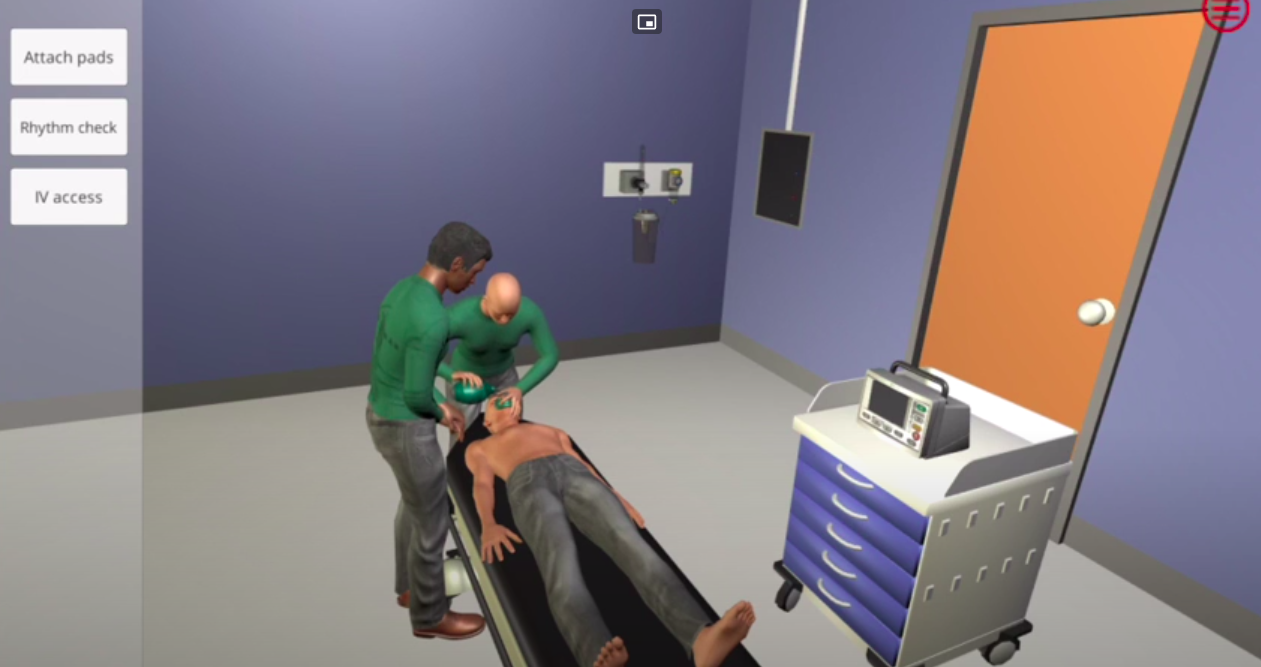
\includegraphics[width=\linewidth]{Virtu-ALS.png}
    \caption{Virtu-ALS}
    \label{fig:virtu-als}
\end{figure}

Virtu-ALS is a \emph{didactic} emergency care simulator developed to teach students and junior healthcare professionals ABCDE assessment protocol \cite{thimInitialAssessmentTreatment2012}, although its application as a reinforcement learning \emph{benchmark} was anticipated and accounted for by the authors \cite{briskAIEnhanceInteractive2018}.
Its most prominent feature is its graphical nature (figure \ref{fig:virtu-als}): the user has access to a 3D-rendered virtual copy of a hospital room, view the monitor, press buttons on a defibrillator, etc.
However, the visual modality means that its observation space 
\begin{equation}
    \obss = \realnums^{307200}
\end{equation}

Such a high dimensionality of the observation space makes it an extremely challenging reinforcement learning task.
Tasks from this family have been solved with deep neural networks \cite{mnihPlayingAtariDeep2013}, however not only does it require a long and expensive training process, it also means that resulting treatment strategies are black box neural networks that no clinical expert understands.
This approach to decision-making is extremely hard to introduce into clinical practice \cite{priceBigDataBlackbox2018,watsonClinicalApplicationsMachine2019}

As our first model, we propose a low-dimensional version of \emph{Virtu-ALS}.
\emph{Auto-ALS} is a modification of Virtu-ALS that removes all the complexity of dealing with a visual 3D environment while retaining all the complexity of dealing with a patient that requires emergency care.
This is achieved by attaching an event listener to Virtu-ALS that registers all observable events that can occur in the simulator in response to the user's actions.
The events are listed in table \ref{tab:auto-als}, organized by which agent action can trigger which event.
\emph{Tick} is a special event that occurs every time the simulator is advanced a timestep, and is negatively reinforced, which when used with reinforcement learning algorithms discourages clinicaly unnecessary actions.

\begin{equation}
     \obs^{+} = \langle \obs_1 \in \obs_1, \exp(\timepoint_1-\timepoint), \dots, \obs_n \in \obs_n, \exp(\timepoint_n-\timepoint), \rangle
\end{equation}

where $\obs_i$ is the value of the observation and $\timepoint$ is current time and $\timepoint_i$ is time when observation $i$ (for $i=5$, \verb|ResponseGroan|) has \emph{last} occurred and $\exp(\timepoint_i-\timepoint)$ represents its decaying relevance.
For \emph{measurements}, the $\obs_i$ equals the magnitude of the measurement, however, for binary obsevations $\obs_i$ would always be equal to one.
For memory efficiency, for all $i$ that correspond to binary observations, $\obs_i$ is skipped from the $o^{+} $ vector and the actual observation vector $o$ has size $36+7*2=50$, as opposed to $36+7)*2=86$

\newpage
\subsection{Decision process}
\label{sec:mpdp}

Implementing Auto-ALS requires grappling with some of the limitations of POMDP framework (as described in section \ref{sec:rlcef})
\begin{enumerate}
    \item Some decision making scenarios legitimately have a discrete flow of time: a CPU, for example, makes a decision every $\frac{1}{\text{clock frequency, Hz}}$ of a second. However, most real-life decision making settings (such as the hospital setting) happen in a continuous time flow with no limits on how often or how rare actions and observations occur.
    \item The agent cannot respond to an observation with less than one (i.e.~zero) or more than one action. This can be fixed by modeling $\action_n)$ as a set of actions.
\end{enumerate}

Both of these problems have been successfully addresed with artificial time discretization and complex action spaces $\actions$, however this is done on a case by case basis for each particular environment. A general model that addresses these challenges would be very useful.

\paragraph{Message Passing Decision Process}

Let us attach a timestamp $\timepoint$ to every observation, reward and action in the decision process, making them 2-tuples. An action $\langle a, \timepoint\rangle$ is a message from the agent to the environment, an observation $\langle \obs, \timepoint \rangle$ or a reward $\langle r, \timepoint \rangle$ is a message from the environment
to the agent. Messages can be sent as often or as rare as needed:

\begin{figure}
\centering

\includegraphics[width=\linewidth]{images/mpdp.png}
\caption{Message Passing Decision Process}
\end{figure}

Observations and actions are sampled from the \emph{environment} and conditioned on the timestamp and all actions of the agent before that time:

\begin{equation}
    \obs_\timepoint \sim p(\obs_\timepoint|\timepoint,\{\action, \timepoint_\action | \timepoint_\action < \timepoint\})
\end{equation}

The actions are sampled from the \emph{agent}, also conditioned on the
timestamp and all observations before that time:

\begin{equation}
a_\timepoint \sim \policy(a_\timepoint|\timepoint, \{ o, \timepoint_o | \timepoint_o < \timepoint \})
\end{equation}

where $\obs_\timepoint \in \obss^{+}$
and $\action_\timepoint \in \actions^{+}$

\begin{equation}
    \obss^{+} = \{\text{no observation} \} \cup \obss
\end{equation}

\begin{equation} 
  \actions^{+} = \{\text{noaction} \} \cup \actions
\end{equation}

\paragraph{Discretization}

Real-world implementation of MPDP 
Now that we're done with the theory, it is a good time to remember that we live in the real world and, in the real world, unless you plan to run reinforcement learning algorithms on a \href{https://royalsocietypublishing.org/doi/10.1098/rstb.2018.0372}{liquid computer} (in which case, please let us know how it goes!), evaluation of $\policy(a_\timepoint)$ will be done either by a regular computer that can only evaluate it a finite number of times a second or something even slower than that. Hence, discretization is still desirable. However, we need a discretization strategy that will make the resulting discrete decision process equivalent (or at least as equivalent as possible) to the continuous MPDP.

\paragraph{Decision schedules}

So we've established that the practicalities of implementing a reinforcement learning algorithm mean that in any timeframe $\langle \timepoint, \timepoint + \Delta \timepoint \rangle$ a finite number of decisions should be taken. This can be achieved by a decision schedule that is some combination of:

\begin{itemize}
\item   making a decision every time any message from the environment   (observation or reward) is received 
\item   making a decision at regular intervals $\Delta \timepoint$ 
\item   after making a decision, scheduling a decision time $\timepoint_d$ later in the future
\end{itemize}

At every decision point the agent has to receive information about the observations that recently occured and output some number of actions (may be zero)

\paragraph{Observation space}

When an observation is modeled as $\langle \obs, \timepoint \rangle$, the most faithful way to represent the history of observations to the agent is

\begin{equation} 
\overrightarrow{\obs} = \langle \obs_1, \timepoint_1, \obs_2, \timepoint_2, \dots \rangle 
\end{equation}

This representation has 2 issues: 
\begin{enumerate}
    \item It has a variable size. There are, of course, machine learning algorithms that can work with variable size inputs \cite{hochreiterLongShorttermMemory1997}, however, most traditional RL approaches cannot and compatibility with them would be an advantage
    \item There is a common type of observation that makes older observations obsolete. For example, in a thermostat a new temperature measurement for all intents and purposes overrides the old one. In a navigation task, a new "location observed" event means you are no longer in the previous location. In Auto-ALS, new measurement of a vital sign, such as heart rate, overrides earlier ones. This has to be taken into account, lest a vast array of outdated information will be fed to the agent at every decision point.
\end{enumerate}

A solution (probably \emph{the} solution?) to these is to sort observations into \emph{observation classes} $\obs_1 \cup \obs_2 \cup \dots \cup \obs_n = O$ such that if several observations from the same class has been made, only the last of them is important. Then $\overrightarrow\{o\}$ should be a vector of the latest observation in each class

\begin{equation} 
  \overrightarrow{o} = \langle \obs_1 \in \obs_1, \exp(\timepoint_1-\timepoint), \dots, \obs_n \in \obs_n, \exp(\timepoint_n-\timepoint), \rangle
\end{equation}

where $\timepoint$ is the decision time. 
$\exp(\timepoint_n-\timepoint)$ is preferable to the more naive approach of $\timepoint-\timepoint_n$, because if no observation in the observation class $\obs_n$ has occurred yet, $\timepoint=-\infty$ which creates all kinds of problems for actually solving the MDP downstream. 
$\exp(\timepoint_n-\timepoint)$ in this case would be simply zero and observations that have occured will have an exponentially decaying relevance factor attached to them - a more directly useful value for decision-making then ``time since event''.

\paragraph{Action space}

Using one of the decision schedules and the observation system described above, it is fairly trivial to support a variable number of actions. 
The agent has to output an action $\action \in \actions$ and if that action is not a "no action", action sampling repeats again.

\newpage
\subsection{Observations}
\label{sec:auto-als-obs}

\texttt{MeasuredHeartRate, MeasuredRespRate, MeasuredCapillaryGlucose, MeasuredTemperature, MeasuredMAP, MeasuredSats, MeasuredResps} are \emph{measurements}, events that have a value $\-infty; +\infty)$ associated with them.

The events in table \ref{tab:auto-als} only get registered if the agent has \emph{learnt} some piece of information, meaning that, for example, \verb|AirwayVomit| will only occur if the patient has vomit in their airway \emph{and} the agent checked the airway (which is part of the standard protocol \cite{thimInitialAssessmentTreatment2012}).
Assessment skills (knowing where to look and how to establish the patient's state) are crucial for patient resuscitation, hence revealing all known health variables to the agent would jeopardize the simulation.

The observation vector in \emph{Auto-ALS} is based on all observations that have occurred between the beginning of the episode and current time.
However, more recent observations are more likely to still be relevant and should be given priority.
This is done with the following formula proposed in section \ref{sec:mpdp}:

\begin{equation}
     o^{+} = \langle \obs_1 \in \obss_1, \exp(\timepoint_1-\timepoint), \dots, \obs_n \in \obss_n, \exp(\timepoint_n-\timepoint), \rangle
\end{equation}

\newpage
\subsection{Actions}
\label{sec:auto-als-act}

\begin{table}[H]
\begin{tabular}{|p{0.4\linewidth}|p{0.45\linewidth}|c|}
\toprule
Agent actions &
  Patient reactions & Rewards
   \\
   \midrule
AssessResponse &
  ResponseVerbal,     ResponseGroan,     ResponseNone &
  \multirow{9}{*}{0} \\
AssessAirway &
  AirwayClear,     AirwayVomit,     AirwayBlood,     AirwayTongue &
   \\
AssessBreathing &
  BreathingNone,     BreathingSnoring,     BreathingSeeSaw,     BreathingEqualChestExpansion,     BreathingBibasalCrepitations,     BreathingWheeze,     BreathingCoarseCrepitationsAtBase,     BreathingPneumothoraxSymptoms,  VentilationResistance, \emph{MeasuredRespRate} &
   \\
AssessCirculation &
  RadialPulsePalpable,     RadialPulseNonPalpable, \emph{MeasuredHeartRate} &
   \\
AssessDisability &
  \verb|AVPU_A|,     \verb|AVPU_U|,     \verb|AVPU_V|, PupilsPinpoint,     PupilsNormal, \emph{MeasuredCapillaryGlucose} &
   \\
AssessExposure &
  ExposureRash,     ExposurePeripherallyShutdown,     ExposureStainedUnderwear, \emph{MeasuredTemperature} &
   \\
AssessDefibrillator &
   &
   \\
AssessMonitor &
  HeartRhythmNSR,
    HeartRhythmSVT,
    HeartRhythmAF,
    HeartRhythmAtrialFlutter,
    HeartRhythmVT,
    HeartRhythmMobitzI,
    HeartRhythmMobitzII,
    HeartRhythmCompleteHeartBlock,
    HeartRhythmTorsades,
    HeartRhythmBigeminy,
    HeartRhythmVF, \emph{MeasuredHeartRate}, \emph{MeasuredMAP}, \emph{MeasuredSats}, \emph{MeasuredResps} &
   \\
   DoNothing & & \\
   \midrule
ABG,     AirwayManoeuvres,     GiveAtropine,     GiveAdenosine,     GiveAdrenaline,     GiveAmiodarone,     GiveMidazolam,     Venflon,     Yankeur,     DrawBloods,     BPCuffOn,     BVM,     Guedel,     NRBMask,     DefibOn,     DefibAttachPads ,     DefibShock,     DefibCharge ,     DefibChangePaceCurrentDown,     DefibChangePaceCurrent,     DefibEnergyDown,     DefibEnergyUp,     DefibChangePaceRateDown,     DefibChangePaceRateUp,     DefibPace& 
   Blunder & $r_\text{blunder}$
   \\
   \midrule
   \multirow{2}{*}{Finish} & Failure & -1 \\
   & Success & 1 \\
   \midrule
   - & Tick & $r_\text{tick}$ \\
  \bottomrule
\end{tabular}
\caption{All actions and observations of Auto-ALS}
\label{tab:auto-als}
\end{table}



We run a program synthesis experiment using SEIDR (see chapter \ref{ch:seidr}) with hyperparameters as desribed in table \ref{tab:rlceps-auto-als}

\begin{table}
    \centering
    \begin{tabular}{|c|c|c|c|c|c|}
        model & $\treearity_\text{draft}$ & $\treearity_\text{explain}$ & $\treearity_\text{debug}$ & $\beamwidth$ & selection \\
        \midrule
        gpt-4o & 3 & 2 & 2 & 5 & tournament
    \end{tabular}
    \caption{Hyperparameter choice for evaluating RLCEPS on Auto-ALS}
    \label{tab:rlceps-auto-als}
\end{table}

\newpage
\section{Auto-ALS results}

\paragraph{Prompts}

Consider the summary table of the ABCDE protocol:

\begin{lstlisting}
+-----------------+---------------------------------------------------+
| Assessment      | Treatment                                         |
+=================+===================================================+
| A – Airways     | Voice                                             |
|                 | Breath sounds                                     |
|                 | Oxygen (15 l min−1) Suction                       |
+-----------------+---------------------------------------------------+
| B – Breathing   | Respiratory rate (12–20 min−1)                    |
|                 | Chest wall movements                              |
|                 | Chest percussion                                  |
|                 | Lung auscultation                                 |
|                 | Pulse oximetry (97%–100%)                         |
+-----------------+---------------------------------------------------+
|                 | Seat comfortably                                  |
|                 | Rescue breaths                                    |
|                 | Inhaled medications                               |
|                 | Bag-mask ventilation                              |
|                 | Decompress tension pneumothorax                   |
+-----------------+---------------------------------------------------+
| C – Circulation | Skin color, sweating                              |
|                 | Capillary refill time (<2 s)                      |
|                 | Palpate pulse rate (60–100 min−1)                 |
|                 | Heart auscultation                                |
|                 | Blood pressure (systolic 100–140 mmHg)            |
|                 | Electrocardiography monitoring                    |
+-----------------+---------------------------------------------------+
|                 | Stop bleeding                                     |
|                 | Elevate legs                                      |
|                 | Intravenous access                                |
|                 | Infuse saline                                     |
+-----------------+---------------------------------------------------+
| D – Disability  | Level of consciousness – AVPU                     |
|                 | Alert                                             |
|                 | Voice responsive                                  |
|                 | Pain responsive                                   |
|                 | Unresponsive                                      |
|                 | Limb movements                                    |
|                 | Pupillary light reflexes                          |
|                 | Blood glucose                                     |
+-----------------+---------------------------------------------------+
|                 | Treat Airway, Breathing, and Circulation problems |
|                 | Recovery position                                 |
|                 | Glucose for hypoglycemia                          |
+-----------------+---------------------------------------------------+
| E - Exposure    | Expose skin                                       |
|                 | Temperature                                       |
+-----------------+---------------------------------------------------+
|                 | Treat suspected cause                             |
+-----------------+---------------------------------------------------+
\end{lstlisting}

Due to the inherent stochasticity of the environment (see chapter \ref{ch:auto-als}) we use 2 tests, which are 2 identical copies of the Auto-ALS environment.
Since lexicase selection assumes multiple deterministic tests, tournament selection is used instead.
We add hard limits on the length of the episode in terms of time (3 hours) as well as steps (350 environment steps).
The initial prompt is as follows:

\lstinputlisting{listings/metanurse_prompt.txt}

and, on iteration 37, the following snippet emerges, that will not be beaten until the end of the experiment (4697 iterations):

\lstinputlisting{listings/auto-als.py}